\begin{frame}[parent={ie:agenda}, hasnext=true, hasprev=false]
	\frametitle{CMMi}

	
	\begin{block:concept}{CMMi}
		Modelo de capacitação de processos de software
	\end{block:concept}
	
	\begin{block:fact}{Organização}
		\begin{itemize}
			\item Organizado em áreas de processo.
			
			\item Cada área de processo define:
			\begin{itemize}
				\item atividades relacionadas,
				\item requisitos para obtenção de um nível no CMMi (metas a serem atendidas)
			\end{itemize}
		\end{itemize}
	\end{block:fact}
	
	\note{Áreas de processo =  antigas KPA - \foreign{Key Process Area}}
\end{frame}


\begin{frame}[hasnext=true, hasprev=true]
	\frametitle{CMMi}

	\begin{block:fact}{CMMi staged}
		\centering
		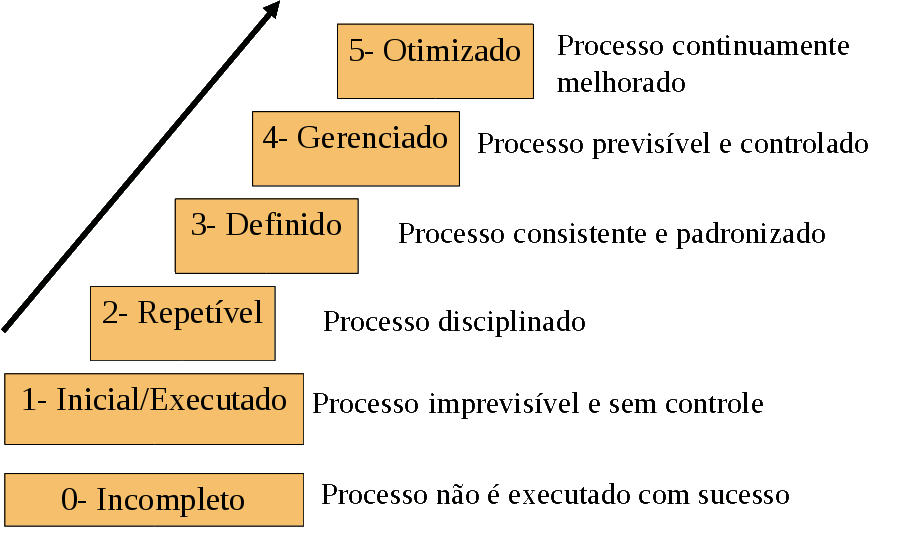
\includegraphics[width=\textwidth]{software-engineering/project-management/process/process-quality/cmmi/cmmi-staged}
	\end{block:fact}
\end{frame}


\begin{frame}
	\frametitle{CMMi}
	\framesubtitle{CMMi staged - Nível 1}
	
	\begin{block:fact}{Nível 1}
		Sucesso é resultado de esforços individuais e heroicos (ou pura sorte)
	\end{block:fact}
	
	\begin{block:fact}{}
		\centering
		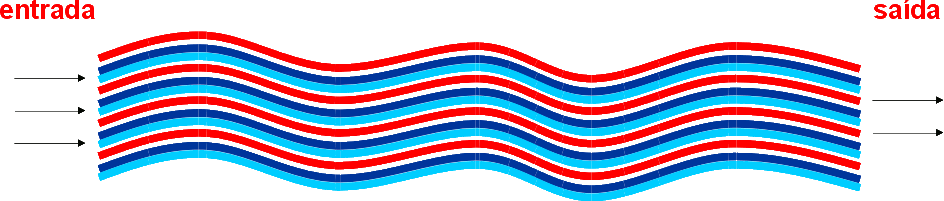
\includegraphics[width=\textwidth]{software-engineering/project-management/process/process-quality/cmmi/cmmi-staged-1}
	\end{block:fact}
\end{frame}


\begin{frame}
	\frametitle{CMMi}
	\framesubtitle{CMMi staged - Nível 1}
	
	\begin{block:fact}{Nível 1}
		Sucesso é resultado de esforços individuais e heroicos (ou pura sorte)
	\end{block:fact}
	
	\begin{block:fact}{Sintomas}
		\begin{itemize}
			\item cronogramas e planos irrealistas
			\item aquilo que é planejado não é seguido (em parte porque eles não tem credibilidade)
			\item cliente só avalia os requisitos no momento da 	entrega
			\item processo de desenvolvimento pula dos requisitos para implementação (para que projeto!)
			\item documentação inexistente
			\item reações contrárias à atividades de melhoria de qualidade
		\end{itemize}
	\end{block:fact}
\end{frame}


\begin{frame}
	\frametitle{CMMi}
	\framesubtitle{CMMi staged - Nível 2}
	
	\begin{block:fact}{Nível 2 -- Repetível}
		\begin{itemize}
		 \item Processo básico de gerência, com controle de custos, prazos e escopo.
		 \item Empresa consegue repetir o sucesso de projetos anteriores em aplicações
		 similares.
		\end{itemize}
	\end{block:fact}
	
	\begin{block:fact}{}
		\centering
		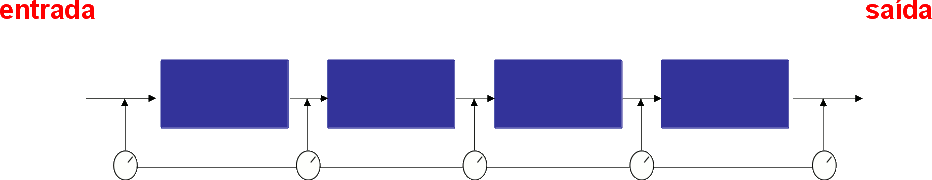
\includegraphics[width=\textwidth]{software-engineering/project-management/process/process-quality/cmmi/cmmi-staged-2}
	\end{block:fact}
\end{frame}


\begin{frame}
	\frametitle{CMMi}
	\framesubtitle{CMMi staged - Nível 2}
	
	\begin{block:fact}{Nível 2 -- Repetível}
		\begin{itemize}
			\item Processo básico de gerência, com controle de custos, prazos e escopo.
			\item Empresa consegue repetir o sucesso de projetos anteriores em aplicações
			similares.
		\end{itemize}
	\end{block:fact}
	
	\begin{block:fact}{Áreas de processo}
		\begin{itemize}
			\small
			\item Gerência de requisitos.
			\item Planejamento de projetos; Monitoramento e controle de projetos.
			\item Garantia de qualidade de processo e de software.
			\item Gerência de contratos com fornecedores.
			\item Gerência de configuração.
			\item Medição e análise.
		\end{itemize}
	\end{block:fact}
\end{frame}

\begin{frame}
	\frametitle{CMMi}
	\framesubtitle{CMMi staged - Nível 2}
	
	\begin{block:fact}{Nível 2 -- Repetível}
		\begin{itemize}
			\item Processo básico de gerência, com controle de custos, prazos e escopo.
			\item Empresa consegue repetir o sucesso de projetos anteriores em aplicações
			similares.
		\end{itemize}
	\end{block:fact}
	
	\begin{block:fact}{Evidências de organizações nível 2:}
		\begin{itemize}
			\item Empresa consegue cumprir compromissos de requisitos, prazos e custos.
			\\No entanto, gerente de projeto não consegue alterar o plano em frente a problemas
			graves.
			\item Evolução controlada dos artefatos de software.
			\item Ainda apresenta resistência às atividades de melhoria de qualidade.
		\end{itemize}
	\end{block:fact}
\end{frame}

\begin{frame}
	\frametitle{CMMi}
	\framesubtitle{CMMi staged - Nível 3}
	
	\begin{block:fact}{Nível 3 -- Definido}
		\begin{itemize}
			\item Processo de software padronizado
			\begin{itemize}
				\item Existe um modelo de processo (processo-padrão) e cada projeto
				utiliza uma versão especializada desse processo
			\end{itemize}
			\item Em cada etapa do desenvolvimento, a organização interna das tarefas
			está definida e visível
		\end{itemize}
	\end{block:fact}
	
	\begin{block:fact}{}
		\centering
		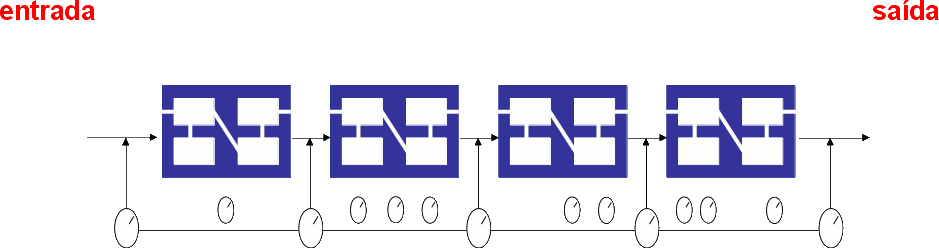
\includegraphics[width=\textwidth]{software-engineering/project-management/process/process-quality/cmmi/cmmi-staged-3}
	\end{block:fact}
\end{frame}

\begin{frame}
	\frametitle{CMMi}
	\framesubtitle{CMMi staged - Nível 3}
	
	\begin{block:fact}{Nível 3 -- Definido}
		\begin{itemize}
			\item Processo de software padronizado
			\begin{itemize}
				\item Existe um modelo de processo (processo-padrão) e cada projeto
				utiliza uma versão especializada desse processo
			\end{itemize}
			\item Em cada etapa do desenvolvimento, a organização interna das tarefas
			está definida e visível
		\end{itemize}
	\end{block:fact}
	
	\begin{block:fact}{Áreas de processo}
		\begin{itemize}
			\small
			\item Gerência de projeto integrada
			\item Definição do processo organizacional
			\item Foco no processo organizacional; Treinamento organizacional
			\item Desenvolvimento de requisitos; Integração do produto
			\item Verificação;  Validação
			\item Gerência de riscos; Análise de decisão e resolução
		\end{itemize}
	\end{block:fact}
\end{frame}

\begin{frame}
	\frametitle{CMMi}
	\framesubtitle{CMMi staged - Nível 3}
	
	\begin{block:fact}{Nível 3 -- Definido}
		\begin{itemize}
			\item Processo de software padronizado
			\begin{itemize}
				\item Existe um modelo de processo (processo-padrão) e cada projeto
				utiliza uma versão especializada desse processo
			\end{itemize}
			\item Em cada etapa do desenvolvimento, a organização interna das tarefas
			está definida e visível
		\end{itemize}
	\end{block:fact}
	
	\begin{block:fact}{Evidências de organizações nível 3}
		\begin{itemize}
			\item Processo padronizado e adaptado para cada projeto.
			\item Abandono de um desenvolvedor não causa prejuízo irreparável ao projeto.
			\item Aplicação de técnicas para melhoria de processo é viável.
		\end{itemize}
	\end{block:fact}
\end{frame}

\begin{frame}
	\frametitle{CMMi}
	\framesubtitle{CMMi staged - Nível 4}
	
	\begin{block:fact}{Nível 4 -- Gerenciado}
		\begin{itemize}
			\item Processo de software padronizado e controlado
			\item Métricas coletadas e utilizadas para gerenciar o projeto
		\end{itemize}
	\end{block:fact}
	
	\begin{block:fact}{}
		\centering
		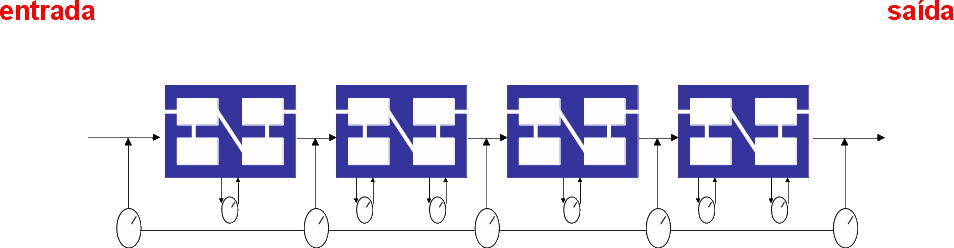
\includegraphics[width=\textwidth]{software-engineering/project-management/process/process-quality/cmmi/cmmi-staged-4}
	\end{block:fact}
\end{frame}


\begin{frame}
	\frametitle{CMMi}
	\framesubtitle{CMMi staged - Nível 4}
	
	\begin{block:fact}{Nível 4 -- Gerenciado}
		\begin{itemize}
			\item Processo de software padronizado e controlado
			\item Métricas coletadas e utilizadas para gerenciar o projeto
		\end{itemize}
	\end{block:fact}
	
	\begin{block:fact}{Áreas de processo}
		\begin{itemize}
			\item Gerência quantitativa dos processos
			\item Desempenho do processo organizacional
		\end{itemize}
	\end{block:fact}
		

	\begin{block:fact}{Evidências de organizações nível 4}
		\begin{itemize}
			\item Organização estabelece metas (quantitativas) para as atividades do
			processo e produtos produzidos
			\item Medidas são coletadas para todos os projetos e para suas atividades
			\item Desvios de execução das atividades são prontamente detectados
		\end{itemize}
	\end{block:fact}
\end{frame}



\begin{frame}
	\frametitle{CMMi}
	\framesubtitle{CMMi staged - Nível 5}
	
	\begin{block:fact}{Nível 5 -- Otimizado}
		\begin{itemize}
			\item Melhoria contínua do processo
			\item Implantação planejada e controlada de melhorias
		\end{itemize}
	\end{block:fact}
	
	\begin{block:fact}{}
		\centering
		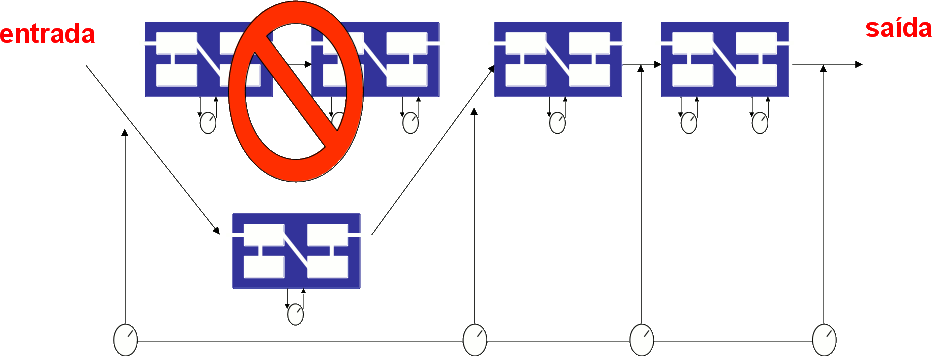
\includegraphics[width=\textwidth]{software-engineering/project-management/process/process-quality/cmmi/cmmi-staged-5}
	\end{block:fact}
\end{frame}


\begin{frame}
	\frametitle{CMMi}
	\framesubtitle{CMMi staged - Nível 5}
	
	\begin{block:fact}{Nível 5 -- Otimizado}
		\begin{itemize}
			\item Melhoria contínua do processo
			\item Implantação planejada e controlada de melhorias
		\end{itemize}
	\end{block:fact}
	
	\begin{block:fact}{Áreas de processo}
		\begin{itemize}
			\item Análise de causas e resolução
			\item Inovação e implantação na organização
		\end{itemize}
	\end{block:fact}


	\begin{block:fact}{Evidências de organizações nível 5}
		\begin{itemize}
			\item Organização engajada em melhoria contínua do processo
			\item Efeitos de cada técnica aplicada são mensuráveis
			\item Para cada melhoria, é possível estabelecer o custo e o benefício
		\end{itemize}
	\end{block:fact}
\end{frame}

\begin{frame}
	\frametitle{CMMi}
	\framesubtitle{Áreas de processo}
	
	\begin{block:fact}{}
		\centering
		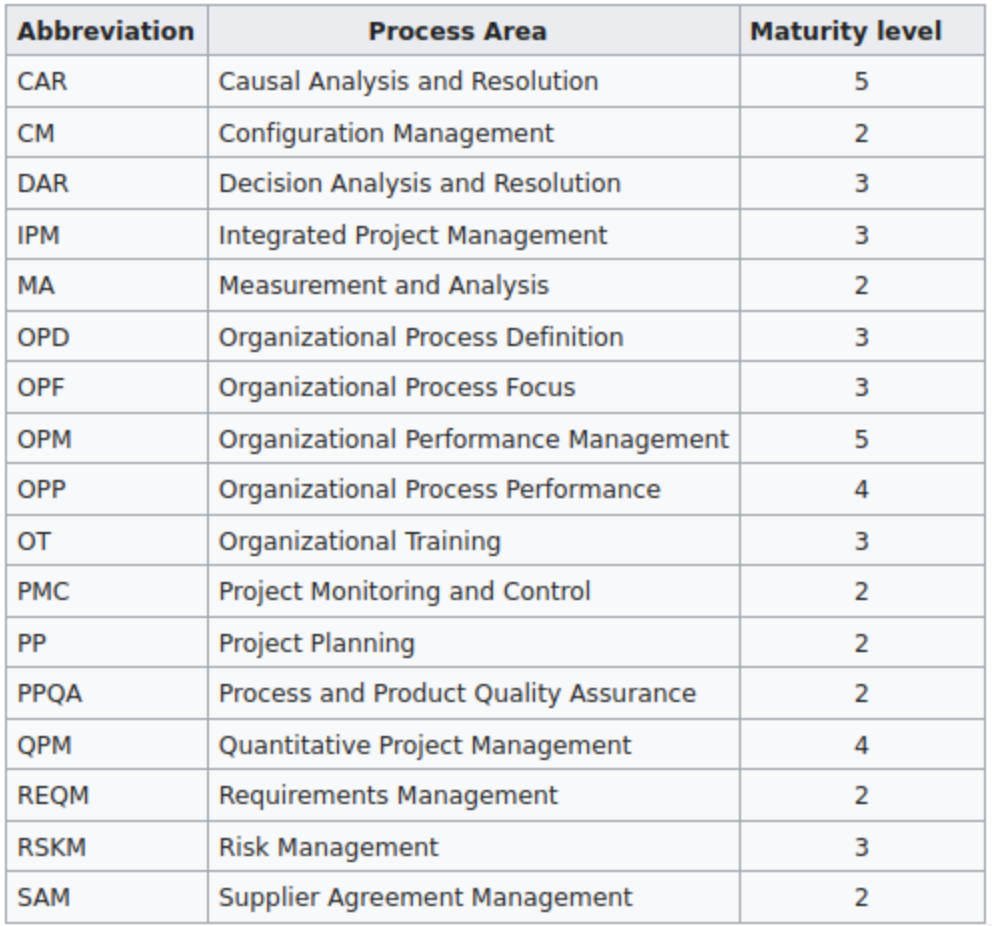
\includegraphics[width=.8\textwidth]{software-engineering/project-management/process/process-quality/cmmi/cmmi-pa}

	\end{block:fact}
\end{frame}


\begin{frame}
	\frametitle{CMMi}
	\framesubtitle{CMMi contínuo}
	
	\begin{block:fact}{Diferença entre contínuo e staged}
		Ao invés de medir a maturidade, é medida a capacidade de uma ou mais áreas
		de processo.
	\end{block:fact}
	
	\begin{block:fact}{}
		\centering
		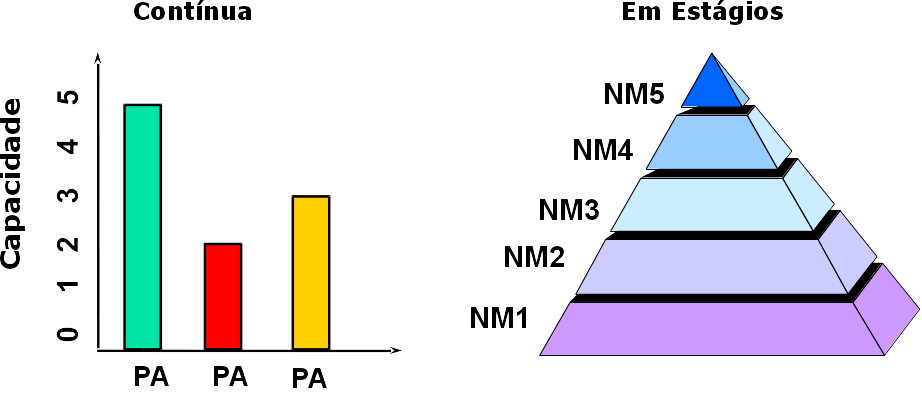
\includegraphics[width=\textwidth]{software-engineering/project-management/process/process-quality/cmmi/cmmi-continuous}
	\end{block:fact}
\end{frame}



\begin{frame}
	\frametitle{CMMi}
	\framesubtitle{Empresas com CMMi}
	
	\begin{block:fact}{}
		\url{https://cmmiinstitute.com/pars}
	\end{block:fact}
	
	\begin{block:fact}{Nível 5 (staged)}
		\begin{itemize}
			\item Critical Software, S.A.
			\item everis
			\item HP Enterprise Services
			\item IBM
			\item Spread Sistemas e Automação Ltda
			\item Synapsis Brasil S.A.
			\item Tata Consultancy Services Limited
		\end{itemize}
	\end{block:fact}

		\begin{block:fact}{Nível 4 (staged)}
		\begin{itemize}
			\item CPM Braxis S.A. (Capgemini)
		\end{itemize}
	\end{block:fact}
\end{frame}

